\documentclass[conference]{IEEEtran}

\usepackage{xcolor} % use colors
\usepackage[utf8]{inputenc} % endoding for i.e. ä, ö and ü
\usepackage[T1]{fontenc} % font encoding
\usepackage{listings} % code listings
\usepackage[font={small, it}]{caption} % adjust caption style
\usepackage{blindtext}
\usepackage{cleveref}
\usepackage{graphicx}

\newcommand{\lref}[1]{listing \ref{#1}}% reference code listings more convenient

%%%%%%%%%%%%%%%%%%%%%%%%%%%%%%%%%%%%%%%%%%%%%%%%%%%%%%%%%%%%%%%%%%%%%%%%%%%%%%%%%%%%%%%%%%
% Java-Style for code listings
%%%%%%%%%%%%%%%%%%%%%%%%%%%%%%%%%%%%%%%%%%%%%%%%%%%%%%%%%%%%%%%%%%%%%%%%%%%%%%%%%%%%%%%%%%
\definecolor{javared}{rgb}{0.6,0,0} % for strings
\definecolor{javagreen}{rgb}{0.25,0.5,0.35} % comments
\definecolor{javapurple}{rgb}{0.5,0,0.35} % keywords
\definecolor{javadocblue}{rgb}{0.25,0.35,0.75} % javadoc
\lstset{%
	language=Java,
	basicstyle=\ttfamily,
	keywordstyle=\color{javapurple}\bfseries,
	stringstyle=\color{javagreen},
	commentstyle=\color{javagreen},
	morecomment=[s][\color{javadocblue}]{/**}{*/},
	numberstyle=\tiny\color{black},
	numbers=left,
	stepnumber=5,
	numbersep=5pt,
	tabsize=2,
	showstringspaces=true,
	breaklines,
	frame=trb,
	captionpos=t,
}
%%%%%%%%%%%%%%%%%%%%%%%%%%%%%%%%%%%%%%%%%%%%%%%%%%%%%%%%%%%%%%%%%%%%%%%%%%%%%%%%%%%%%%%%%%
% Other settings for code listings
%%%%%%%%%%%%%%%%%%%%%%%%%%%%%%%%%%%%%%%%%%%%%%%%%%%%%%%%%%%%%%%%%%%%%%%%%%%%%%%%%%%%%%%%%%
\lstset{
	literate=%
	{Ö}{{\"O}}1
	{Ä}{{\"A}}1
	{Ü}{{\"U}}1
	{ß}{{\ss}}1
	{ü}{{\"u}}1
	{ä}{{\"a}}1
	{ö}{{\"o}}1
	{~}{{\textasciitilde}}1
}

%%%%%%%%%%%%%%%%%%%%%%%%%%%%%%%%%%%%%%%%%%%%%%%%%%%%%%%%%%%%%%%%%%%%%%%%%%%%%%%%%%%%%%%%%%
% Document title
%%%%%%%%%%%%%%%%%%%%%%%%%%%%%%%%%%%%%%%%%%%%%%%%%%%%%%%%%%%%%%%%%%%%%%%%%%%%%%%%%%%%%%%%%%
\title{Assignment 2 - Internal Softare Quality}

%%%%%%%%%%%%%%%%%%%%%%%%%%%%%%%%%%%%%%%%%%%%%%%%%%%%%%%%%%%%%%%%%%%%%%%%%%%%%%%%%%%%%%%%%%
% Authors
%%%%%%%%%%%%%%%%%%%%%%%%%%%%%%%%%%%%%%%%%%%%%%%%%%%%%%%%%%%%%%%%%%%%%%%%%%%%%%%%%%%%%%%%%%
\author{\IEEEauthorblockN{Heiko Joshua Jungen}
	\IEEEauthorblockA{
		Software Engineering\\
		Chalmers University of Technology\\
		Sweden, Gothenburg\\
		Email: jungen@student.chalmers.se
	}
	\and
	\IEEEauthorblockN{David Fogelberg}
	\IEEEauthorblockA{
		Software Engineering\\
		Chalmers University of Technology\\
		Sweden, Gothenburg\\
		Email: fodavid@student.chalmers.se
}}

%%%%%%%%%%%%%%%%%%%%%%%%%%%%%%%%%%%%%%%%%%%%%%%%%%%%%%%%%%%%%%%%%%%%%%%%%%%%%%%%%%%%%%%%%%
% Start of document
%%%%%%%%%%%%%%%%%%%%%%%%%%%%%%%%%%%%%%%%%%%%%%%%%%%%%%%%%%%%%%%%%%%%%%%%%%%%%%%%%%%%%%%%%%
\begin{document}
\maketitle
\tableofcontents

%%%%%%%%%%%%%%%%%%%%%%%%%%%%%%%%%%%%%%%%%%%%%%%%%%%%%%%%%%%%%%%%%%%%%%%%%%%%%%%%%%%%%%%%%%
\begin{abstract}
    In this paper measured and human perceived complexity of source code is discussed. It outlines how complexity is perceived by humans and compares it to measured complexity. Further, ...
\end{abstract}

%%%%% DAVID %%%%%%%%%%%%%%%%%%%%%%%%%%%%%%%%%%%%%%%%%%%%%%%%%%%%%%%%%%%%%%%%%%%%%%%%%%%%%%%%%%%%%
\section{Introduction}

In this report five open source Java projects are compared by using their internal qualities. The five projects are: Amazequest, Umlet, Expr, BscSoftware and uHabits. SourceMonitor was used as an measurment tool for measuring the different internal quality factors. The different comparisons between the internal qualities will be discussed below.  

%%%%%%%%%%%%%%%%%%%%%%%%%%%%%%%%%%%%%%%%%%%%%%%%%%%%%%%%%%%%%%%%%%%%%%%%%%%%%%%%%%%%%%%%%%
\section{Perceived and measured complexity }

%%%%%%%%%%%%%%%%%%%%%%%%%%%%%%%%%%%%%%%%%%%%%%%%%%%%%%%%%%%%%%%%%%%%%%%%%%%%%%%%%%%%%%%%%%
\subsection{Ranking of perceived complexity}
\label{ssec:ranking}
% reference a listing -> \lref{method:getAngle}
In this section five methods are compared and ranked by their perceived complexity, where value one is the highest rank. The perceived complexity for a method is determined by looking at cohesion, coupling, documentation and understandability of method names and variable names. Cohesion is seen as one of the most critical factors since a low cohesion leads to a method that does more than its main task. This makes it harder to understand what a method does since every task, including the main task, needs to be analyzed in order to get a clear view. Coupling is also seen as one of the most critical factors since a tightly coupled method is dependent on other methods. In order to understand what a tightly coupled method does, an analyze of the dependent methods are also needed. Meanwhile documentation and the understandability of method names and variable names are seen as less critical when determining the perceived complexity for a method. The reason for this is because even if a documentation is well written and all the names are clear in a method, the reader can still struggle to understand what is happening when for example there is low cohesion. Methods with low cohesion and tight coupling will therefore be perceived as more complex when doing a pairwise comparison. An example of this is the draw method that gets rank one while the getAngle method gets rank five because of the differences in coupling and cohesion, see \cref{tbl:ranking}. Even if the variables names are more vague in the getAngle method then the draw method, it is easier to understand what the method does and therefore the draw method gets an higher complexity. 

%%%%%%%%%%%%%%%%%%%%%%%%%%%%%%%%%%%%%%%%%%%%%%%%%%%%%%%%%%%%%%%%%%%%%%%%%%%%%%%%%%%%%%%%%%
% Ranking table
%%%%%%%%%%%%%%%%%%%%%%%%%%%%%%%%%%%%%%%%%%%%%%%%%%%%%%%%%%%%%%%%%%%%%%%%%%%%%%%%%%%%%%%%%%

\begin{table}
\centering
	\begin{tabular}{c | l l}
		Rank 	& Measured complexity   & Perceived complexity      \\ \hline 
		1 		& intersect	            & draw                      \\ 
		2 		& getAngle       	    & checkKeyword              \\ 
		3 		& checkKeyword  	    & intersect                 \\ 
		4 		& getParameters         & getParameters             \\ 
		5 		& draw 		            & getAngle                  \\ 
	\end{tabular} 
\caption{This table shows the ranking of measured and perceived complexity for the selected method. Measured complexity is shown in descending order of the measured complexity value in the second column. The order of perceived complexity is shown in the third column. In both columns rank 1 is the most and rank 5 the least complex.}
\label{tbl:ranking}
\end{table}

%%%%%%%%%%%%%%%%%%%%%%%%%%%%%%%%%%%%%%%%%%%%%%%%%%%%%%%%%%%%%%%%%%%%%%%%%%%%%%%%%%%%%%%%%%
\subsection{Comparison to measured complexity}
\label{ssec:comparison}
This section compares the perceived and measured complexity, and concludes about the quality of the latter one. First of all, the criteria for calculating the complexity are presented and compared to criteria for perceived complexity, which are discussed in \cref{ssec:ranking}. Finally, the quality of the measured complexity is elaborated.

Measured complexity is calculated by an algorithm according to the following criteria. At the beginning the complexity of a method is 1. This value increases by 1 for every conditional statement (i.e. if, else, for, while) and further increases by 1 for additional logical statements of the conditional statements (i.e '\&\&', '||'). Hence, the measured complexity linearly increases with every conditional and logical statement. Defining a reasonable threshold for the measured complexity value limits the amount of branches in a method. In order to not exceed the threshold developers would have to simplify code, or extract parts of the method in subroutines, which may comforts the ease to understand source code.

Human perceived complexity differs greatly from the before presented measured complexity. The algorithm for measuring complexity determines the number of execution paths and results with a value of measured complexity, hence it takes a single aspect into account to express complexity. Unlike this, human perceived complexity is the result of multiple aspects and additionally a subjective decision with no fixed value. It depends on the technical knowledge of the reader and may vary noticeable. When reading method source code, the reader needs to understand what is happening in order to perceive the method as not complex. Vague method or variable names decrease the ease of understanding, too many subroutines require more reading effort, and multiple actions within a method may overload the readers grasping capabilities. Additionally, readers with greater technical or domain knowledge may understand more difficult source code, whereas readers without said knowledge would not capable to understand. 

In direct comparison of the measured and perceived complexity of the selected methods the differences become more clear. For instance according to \cref{tbl:ranking}, the draw-method is measured as not very complex, although it is perceived as the most complex. In this method the measured complexity is low, because the method contains just a single conditional statement (see line 16 in \lref{method:draw}). However, various method calls, the usage of global variables and performing multiple actions subsequently the method appears complex to humans. Another interesting outcome is the comparison of the getAngle-method. Measuring the complexity of this method by counting the execution paths results in the second biggest measured complexity value. Anyhow, in the ranking of human perceived complexity it is considered the least complex method. The source code shows various conditional statements with multiple logical statements within (see lines 9, 12, 15 and 18 in \lref{method:getAngle}), hence the measured complexity value increases often. But the method is focused on a single task and does not call many subroutines, which makes it easy to understand its purpose and what is happening.

In conclusion, perceived complexity is more complicated than measured complexity, because it is subjective and takes multiple aspects into account. In contrast to the perceived complexity, the presented measured complexity focuses solely on the total number of execution paths. For that reason, measured complexity is not sufficient enough to represent the actual human perceived complexity. Although, this may not hint that measured complexity is bad, but rather is not sufficient to represent human perception on its own. Thresholds for the complexity value will limit the number of conditional and related logical statements, hence will support the ease of understanding. That being said, additional measures should be taken into account to express the actual complexity, because human perception is not based on one aspect as well. Considering measurements for method coupling and cohesion would support a more accurate statement about actual complexity. Anyhow, aspects like understandable method and variable names as well as technical knowledge are hard to examine for an algorithm. Summarising, applying thresholds for measured complexity may decrease human perceived complexity, though it is most certainly not a guarantor, but rather one aspect of a more difficult subject.

%%%%%%%%%%%%%%%%%%%%%%%%%%%%%%%%%%%%%%%%%%%%%%%%%%%%%%%%%%%%%%%%%%%%%%%%%%%%%%%%%%%%%%%%%%
\section{Internal quality}

\subsection{Measurements metrics and thresholds}
% Metrics: Nested depth, Complexity, Method calls,
This section introduces the chosen measurements and respective thresholds used to estimate the internal quality of the products. Nested depth, complexity and method calls are the chosen measurements to conclude about the internal quality. The first measurement, namely Nested depth, is the maximum counted number of nested conditional statements within a method. Complexity of a method is expressed by an integer value, that is the higher the more conditional and logical statements the method has. Thereby, the default value is 1 and it increases by 1 for every conditional or logical statements. The last measurement is the number of method calls within the examined method. 

% Thresholds
Estimation of internal software quality by using said measurements requires a definition of what is good and bad quality. For that reason, every measurement needs a threshold, that when exceeded stand for bad quality. The threshold values for the maximum depth, complexity and method calls are shown in \cref{tbl:thresholds} and are based upon recommendation from literature or experience.
\begin{table}
\centering
    \begin{tabular}{c c}
         Metric         & Threshold    \\ \hline
         Maximum depth  & 7             \\
         Complexity     & 10            \\
         Method calls   & 20            \\
    \end{tabular}
    \caption{This table shows the threshold for the selected metrics}
    \label{tbl:thresholds}
\end{table}

\begin{table*}
\centering
\begin{tabular}{l|c c c c c c c}
	Project     & Depth & Rel. depth & Complexity & Rel. complexity & Calls & Rel. Calls & Number of methods \\ \hline
	AmazeQuest  &   0   & 0,00       & 0          & 0,00            & 3     & 0,03       & 90                \\
	BscSoftware &   2   & 0,003      & 3          & 0,01            & 13    & 0,02       & 577               \\
	Expr        &   0   & 0,00       & 1          & 0,02            & 4     & 0,06       & 64                \\
	uHabits     &   0   & 0,00       & 4          & 0,00            & 62    & 0,03       & 1888              \\
	UMLet       &  31   & 0,01       & 18         & 0,01            & 156   & 0,05       & 3408
\end{tabular} 
\caption{This table shows the absolute and relative number of methods that exceed the threshold for maximum depth, complexity, or methods calls. The relative value is calculating by the number of methods within the respective project.}
\label{tbl:exceed}
\end{table*}

\subsection{Analysis of measurement metrics}
% diagrams

% Describe exceed depth here.. %%%%%%%%%%%%%%%%%%%%%%%%%%%%%   
The diagram in \cref{fig:exceed_depth} shows the projects relative depth on method level, which is in this case a percent measure of how many methods that have a nested depth greater than seven. The relative depth is shown on the y-axis for each project and the project names are shown on the x-axis. According to this diagram, the UMLet project is seen as more complex since it   has the highest relative depth value compared to the other projects. This is reasonable because if a lot of methods in a project has a nesting depth that is very large, the methods in that project become difficult to understand, which also leads to difficulty in maintaining that project. 
\begin{figure}
    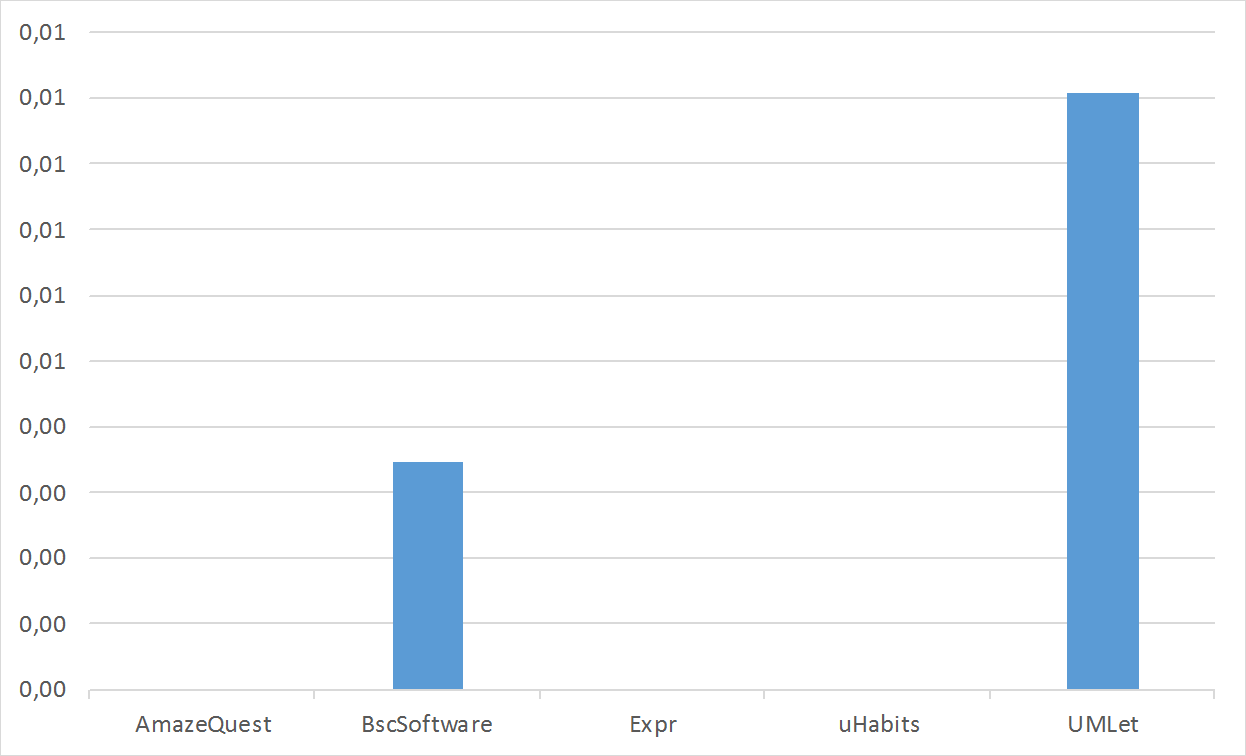
\includegraphics[width=\columnwidth]{img/rel_exceeded_depth.png}
\caption{Relative exceeded maximum depth.}
\label{fig:exceed_depth}
\end{figure}

% Describe complexity here.. %%%%%%%%%%%%%%%%%%%%%%%%%%%%%

\begin{figure}
	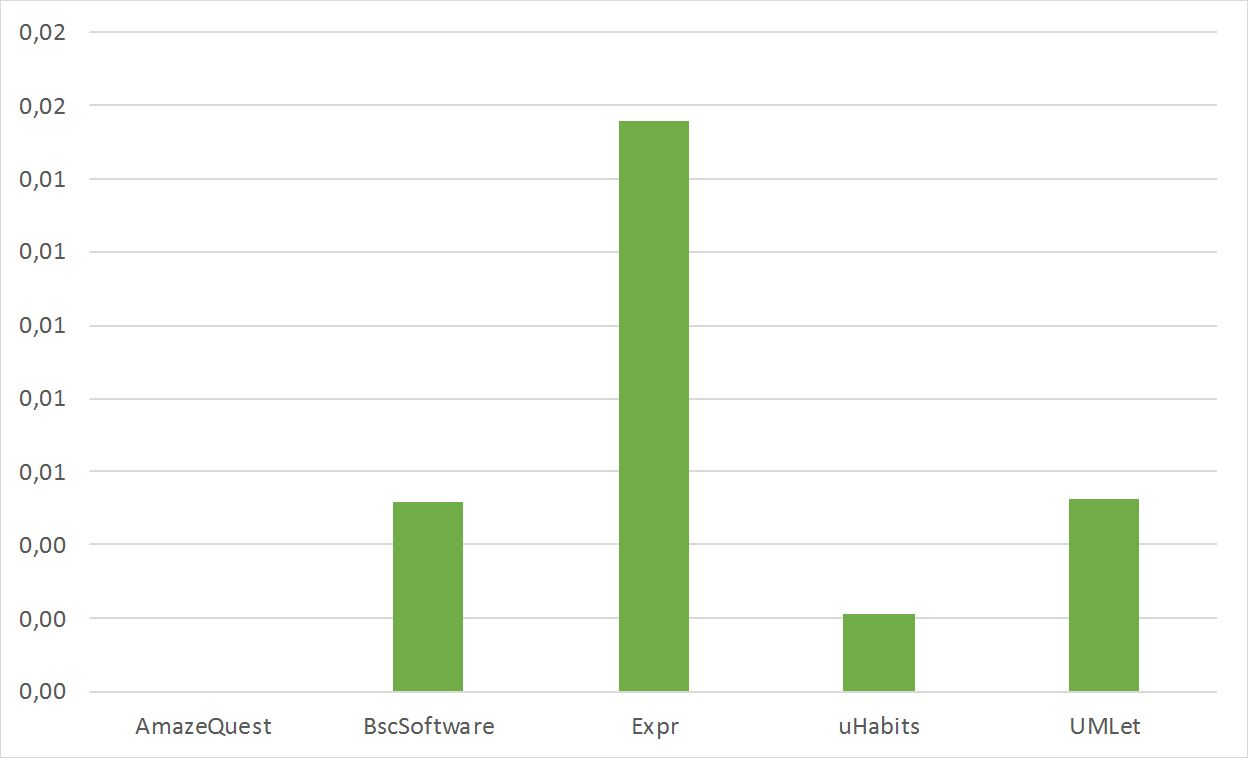
\includegraphics[width=\columnwidth]{img/rel_exceeded_complexity.png}
\caption{Relative exceeded complexity.}
\label{fig:exceed_complexity}
\end{figure}

% Describe exceed calls here..%%%%%%%%%%%%%%%%%%%%%%%%%%%%%   work work 
\begin{figure}
	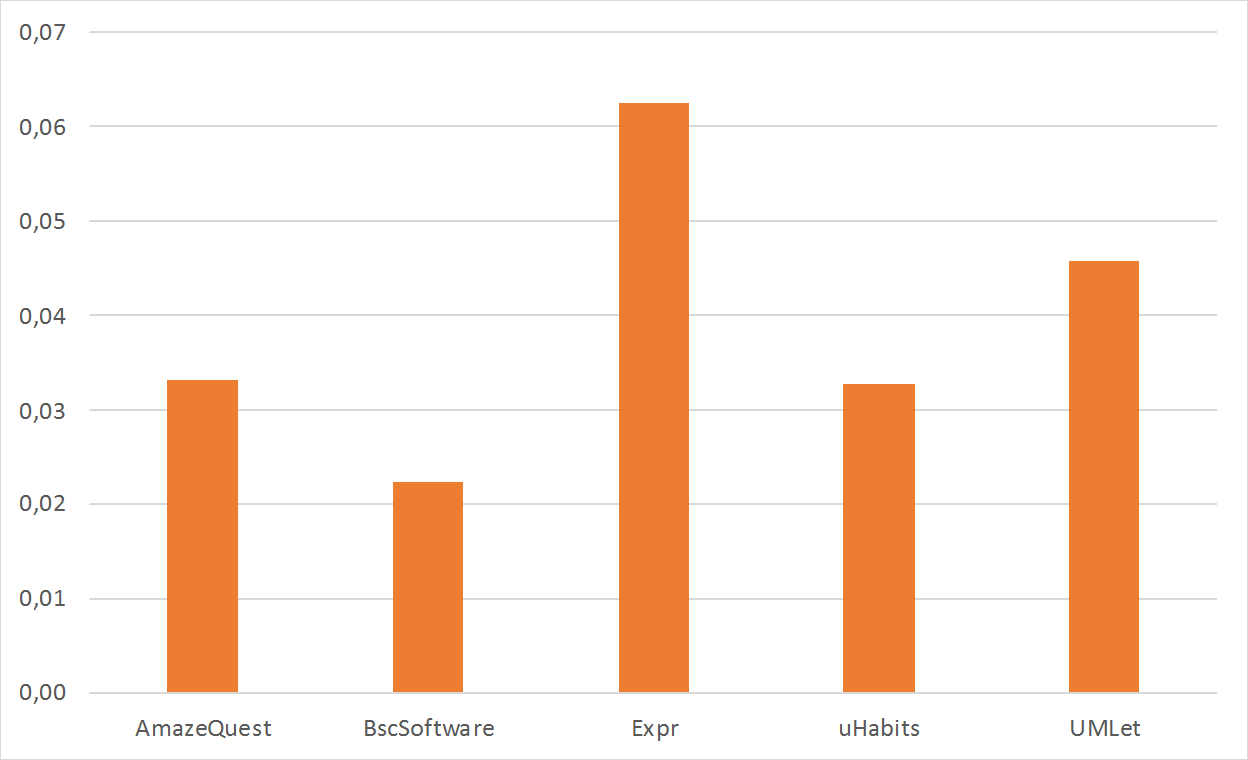
\includegraphics[width=\columnwidth]{img/rel_exceeded_calls.png}
\caption{Relative exceeded method calls.}
\label{fig:exceed_calls}
\end{figure}
% weight of metric

\subsection{Conclusion}

%%%%%%%%%%%%%%%%%%%%%%%%%%%%%%%%%%%%%%%%%%%%%%%%%%%%%%%%%%%%%%%%%%%%%%%%%%%%%%%%%%%%%%%%%%
\section{Refactoring}


%%%%%%%%%%%%%%%%%%%%%%%%%%%%%%%%%%%%%%%%%%%%%%%%%%%%%%%%%%%%%%%%%%%%%%%%%%%%%%%%%%%%%%%%%%
\section{Acknowledgement}

%%%%%%%%%%%%%%%%%%%%%%%%%%%%%%%%%%%%%%%%%%%%%%%%%%%%%%%%%%%%%%%%%%%%%%%%%%%%%%%%%%%%%%%%%%
\section{Conclusion}

\appendix
\section{Code Listings}

\lstinputlisting[float=*, language=Java, 
    caption={
    	The listing shows the source code of the draw-method. Perceived complexity is high, because the method relies on several other methods and global variables. Further, low cohesion and lack of comments additionally increase the human perceived complexity level. The    measured complexity for this method is 2.}, 
    label={method:draw}]
{code/method_draw.java}

\lstinputlisting[float=*, language=Java, 
    caption={
        That listing presents the checkKeyword-method source code. The absence of sufficient documentation, vague method and variable names, as well as low cohesion are making the perceived complexity relatively high. The measured complexity value is 6.},
    label={method:checkKeyword}]
{code/method_checkKeyword.java}

\lstinputlisting[float=*, language=Java, 
    caption={
    	This code listing contains the intersect-method. It is loosely coupled and the variable names are easy to understand. However, the perceived complexity is increased by low cohesion, because the method performs two actions at the same time (calculating a minimum and maximum value). The measured complexity for this method is 11.}, 
    label={method:intersect}]
{code/method_intersect.java}

\lstinputlisting[float=*, language=Java, 
    caption={
        Here the source code of the getParameters-Method is shown. The method lacks understandable variable names and proper documentation, but due to high cohesion and loose coupling the perceived complexity is relatively low. The measured complexity for this method is 4.}, 
    label={method:getParameters}]
{code/method_getParameters.java}

\lstinputlisting[float=*, language=Java, 
    caption={
        This listing contains the source code of the getAngle-method. Although it lacks sufficient documentation and meaningful variable names, the high cohesion and low coupling keeps the perceived complexity very low. The measured complexity value is 9.},
    label={method:getAngle}]
{code/method_getAngle.java}
	
\end{document}
